\documentclass[border=10pt]{standalone}
\usepackage[svgnames]{xcolor}
\usepackage{amsmath}
\usepackage{pgfplots}
\pgfplotsset{compat=newest}
\usepackage[sfdefault]{FiraSans}
\usepackage{FiraMono}
\renewcommand*\familydefault{\sfdefault}
\begin{document}
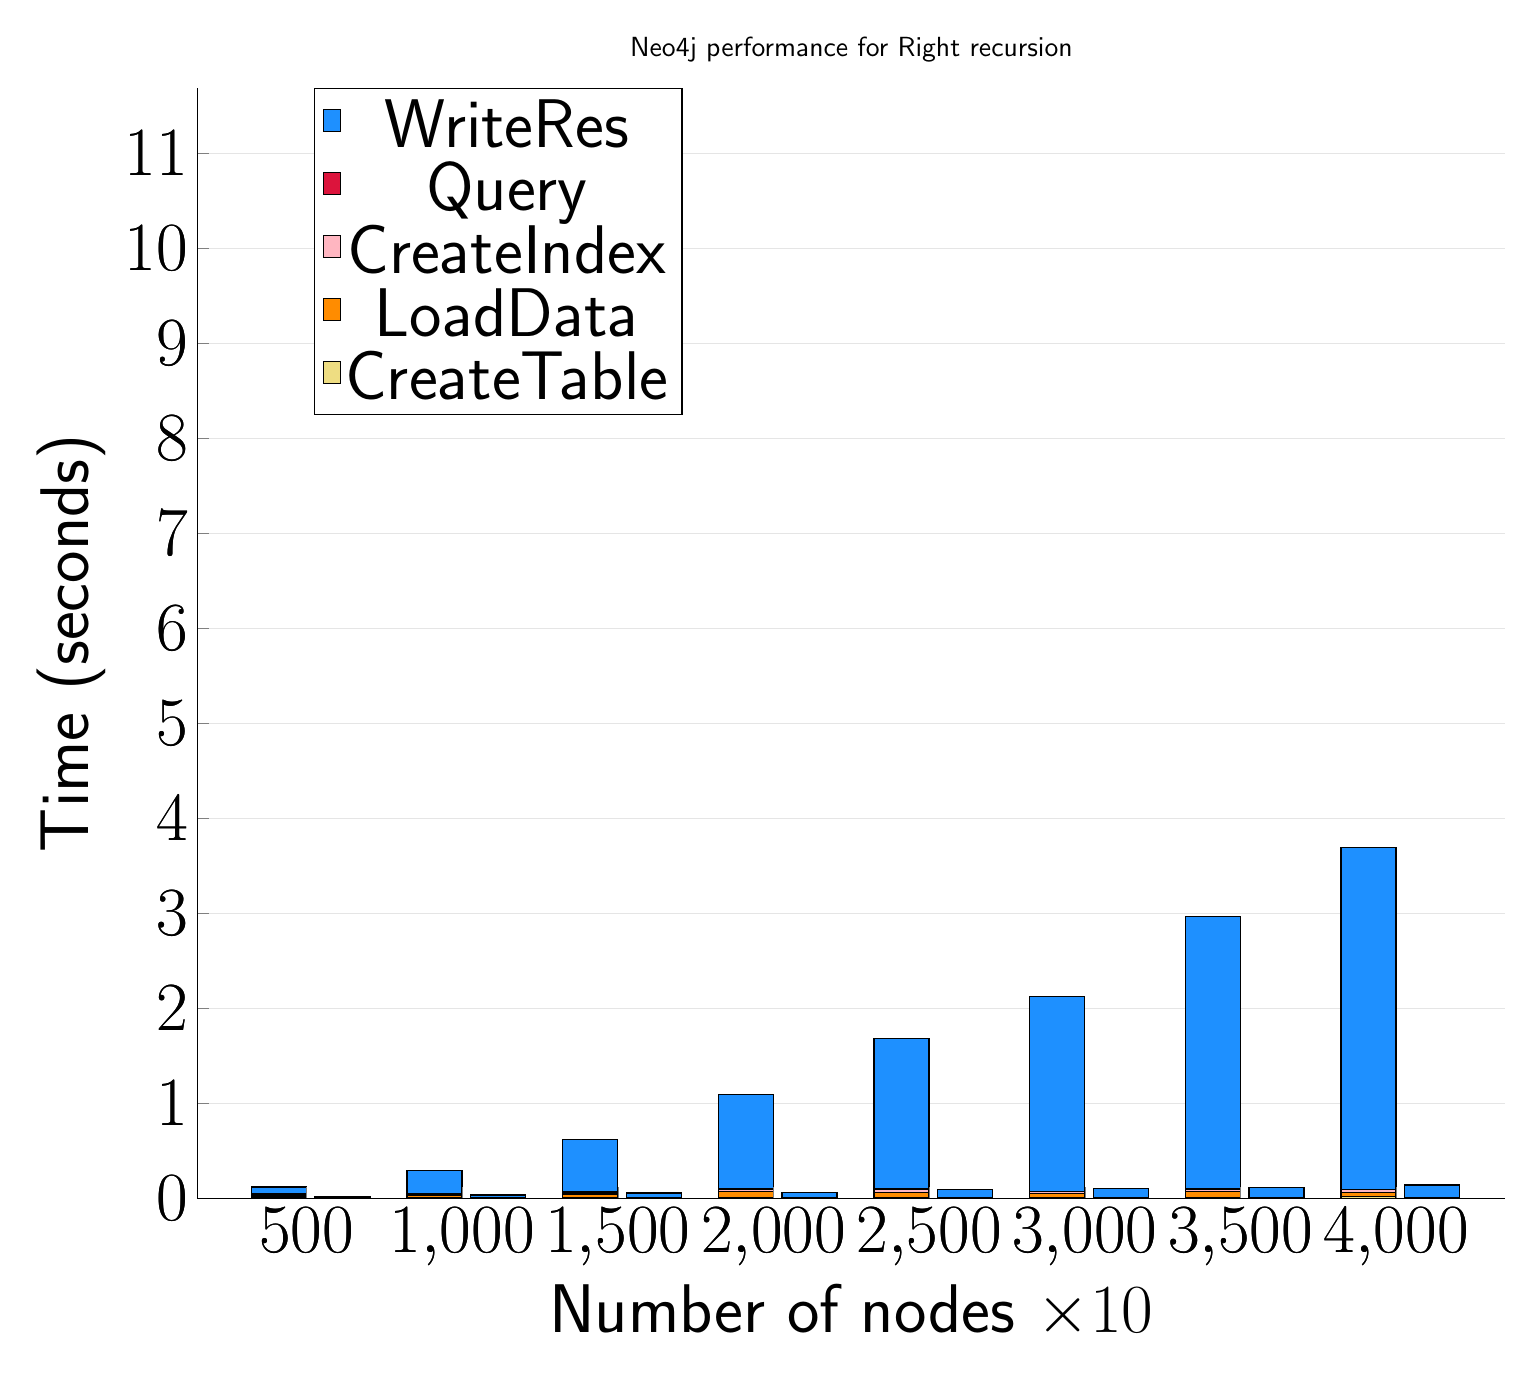
\begin{tikzpicture}
\begin{axis}[
   ybar stacked,
   title={Neo4j performance for Right recursion},
   bar shift=-10pt,
   width=1.5\textwidth,
   bar width=0.7cm,
   ymajorgrids, tick align=inside,
   major grid style={draw=gray!20},
   xtick=data,
   ymin=0, ymax=11.693333332737287,
   axis x line*=bottom,
   axis y line*=left,
   enlarge x limits=0.1,
   legend style={
       at={(0.23, 1)},
       anchor=north,
       legend columns=1,
       font=\Huge,
   },
   ylabel={Time (seconds)},
   xlabel={Number of nodes $\times 10$},
   label style={font=\Huge},
   tick label style={font=\Huge},
]
\addlegendimage{fill=DodgerBlue, draw=black, line width=0.2pt}
\addlegendentry{WriteRes}
\addlegendimage{fill=Crimson, draw=black, line width=0.2pt}
\addlegendentry{Query}
\addlegendimage{fill=LightPink, draw=black, line width=0.2pt}
\addlegendentry{CreateIndex}
\addlegendimage{fill=DarkOrange, draw=black, line width=0.2pt}
\addlegendentry{LoadData}
\addlegendimage{fill=LightGoldenrod, draw=black, line width=0.2pt}
\addlegendentry{CreateTable}
\addplot +[fill=LightGoldenrod, draw=black, line width=0.5pt] coordinates {
    (500, 0.01333333303531011)
    (1000, 0.009999997913837433)
    (1500, 0.013333330551783243)
    (2000, 0.01333333303531011)
    (2500, 0.013333330551783243)
    (3000, 0.013333330551783243)
    (3500, 0.01333333800236384)
    (4000, 0.019999998311201733)
};
\addplot +[fill=DarkOrange, draw=black, line width=0.5pt] coordinates {
    (500, 0.010000000397364298)
    (1000, 0.026666668554147083)
    (1500, 0.033333333830038704)
    (2000, 0.05999999990065893)
    (2500, 0.050000001986821495)
    (3000, 0.04000000158945719)
    (3500, 0.05999999741713206)
    (4000, 0.04333333422740301)
};
\addplot +[fill=LightPink, draw=black, line width=0.5pt] coordinates {
    (500, 0.013333335518836975)
    (1000, 0.01333333303531011)
    (1500, 0.023333335916201275)
    (2000, 0.019999998311201733)
    (2500, 0.02999999870856603)
    (3000, 0.020000000794728596)
    (3500, 0.026666668554147087)
    (4000, 0.030000001192092896)
};
\addplot +[fill=Crimson, draw=black, line width=0.5pt] coordinates {
    (500, 0.01333333303531011)
    (1000, 0.0)
    (1500, 0.0)
    (2000, 0.013333335518836975)
    (2500, 0.010000000397364298)
    (3000, 0.0)
    (3500, 0.0)
    (4000, 0.0)
};
\addplot +[fill=DodgerBlue, draw=black, line width=0.5pt] coordinates {
    (500, 0.07333333293596904)
    (1000, 0.2433333322405815)
    (1500, 0.5500000019868215)
    (2000, 0.9866666669646899)
    (2500, 1.5833333333333333)
    (3000, 2.0566666647791862)
    (3500, 2.8666666646798453)
    (4000, 3.5999999990065894)
};
\end{axis}
\begin{axis}[
   ybar stacked,
   bar shift=13pt,
   width=1.5\textwidth,
   bar width=0.7cm,
   ymajorgrids, tick align=inside,
   major grid style={draw=none},
   xtick=data,
   ymin=0, ymax=11.693333332737287,
   axis x line*=none,
   axis y line*=none,
   enlarge x limits=0.1,
   label style={font=\Huge},
   tick label style={font=\Huge},
]
\addplot +[fill=LightGoldenrod, draw=black, line width=0.5pt] coordinates {
    (500, 0.003333333333333337)
    (1000, 0.003333333333333337)
    (1500, 0.010000000000000007)
    (2000, 0.0)
    (2500, 0.003333333333333336)
    (3000, 0.010000000000000005)
    (3500, 0.006666666666666674)
    (4000, 0.003333333333333336)
};
\addplot +[fill=DarkOrange, draw=black, line width=0.5pt] coordinates {
    (500, 0.0)
    (1000, 0.003333333333333336)
    (1500, 0.0)
    (2000, 0.0)
    (2500, 0.0)
    (3000, 0.0)
    (3500, 0.0)
    (4000, 0.0)
};
\addplot +[fill=LightPink, draw=black, line width=0.5pt] coordinates {
    (500, 0.0066666666666666515)
    (1000, 0.0)
    (1500, 0.0)
    (2000, 0.010000000000000007)
    (2500, 0.0)
    (3000, 0.0)
    (3500, 0.0)
    (4000, 0.003333333333333336)
};
\addplot +[fill=Crimson, draw=black, line width=0.5pt] coordinates {
    (500, 0.0)
    (1000, 0.0)
    (1500, 0.0)
    (2000, 0.003333333333333336)
    (2500, 0.006666666666666668)
    (3000, 0.0)
    (3500, 0.0)
    (4000, 0.006666666666666672)
};
\addplot +[fill=DodgerBlue, draw=black, line width=0.5pt] coordinates {
    (500, 0.00999999999999999)
    (1000, 0.02999999999999998)
    (1500, 0.04666666666666667)
    (2000, 0.05333333333333331)
    (2500, 0.08333333333333333)
    (3000, 0.09333333333333331)
    (3500, 0.10666666666666663)
    (4000, 0.13)
};
\end{axis}
\end{tikzpicture}

\end{document}
